% \begin{figure}
% 	\chapter{Приложение 2. Построенная нечеткая когнитивная карта}\label{nfcm}

% 	\begin{center}
% 	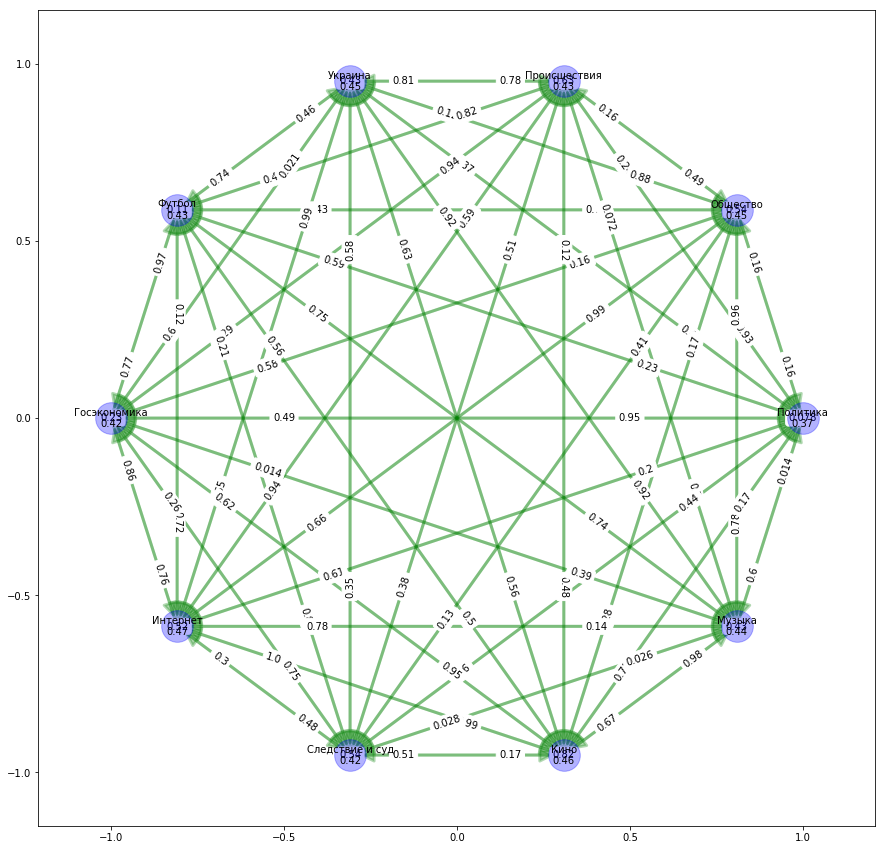
\includegraphics[width=.9\columnwidth]{./img/nfcm.png}
% 	\end{center}
% 	\caption{Построенная нечеткая когнитивная карта}%
% 	\label{pic:nfcm}%
% \end{figure}


% % \chapter{Общая структура пояснительной записки}\label{app-structure}
% % %\addcontentsline{toc}{chapter}{}

% % \begin{enumerate}
% % 	\item Титульный лист %(в данном примере используется титульный лист от преддипломной практики)
% % 	\item Лист с подписями (только для ВКР)
% % 	\item Задание (в данном примере используется задание на диплом)
% % 	\item Отчет из Интиплагиага \footnote{Обычно, допускается до 30\% заимствованного текста для работ бакалавров и до 20\% -- для работ магистров; см. соответствующие нормативные документы}
% % 	\item Реферат (всегда на отдельной стр.)%, и эта страница \textit{НЕ} нумеруется)
% % 	\item Оглавление. Начинается с новой страницы. %Обычно, это первая нумеруемая страница.
% % 	\item Введение
% % 	\begin{enumerate}
% % 		\item Актуальность
% % 		\item Новизна
% % 		\item Оригинальная суть исследования
% % 		\item Содержание ПЗ по главам (тезисно)
% % 	\end{enumerate}
% % 	\item Аналитическая глава. Пишется в стиле \textit{аналитического обзора}
% % 	\item Теоретическая и инженерная глава. Описываются использованные, доработанные и разработанные модели, алгоритмы, методы, и т.п. Кроме того, тут формулируется архитектура системы.
% % 	\item Инженерная глава. В этой главе следует отразить результаты проектирования, что, в общем случае, включает в себя следующие пункты:
% % 	\begin{enumerate}
% % 		\item Описание используемой методики проектирования
% % 		\item Общая архитектура системы
% % 		\item Архитектура подсистемы [таких подразделов может быть несколько штук, по одному на каждую подсистему или модуль, требующую детальное рассмотрение]
% % 		\item Проектирование внешних и внутренних интерфейсов/протоколов взаимодействия
% % 	\end{enumerate}
% % 	\item Практическая глава. Описывается реализация, включая выбор инструментальных средств \footnote{В тех случаях, когда \begin{inparaenum}[(a)]\item этот выбор имеет существенное значение для всей работы и \item он не был, по каким-либо причинам, проделан в аналитической главе \end{inparaenum}}. Типовое содержание:
% % 	\begin{enumerate}
% % 		\item Состав и структура реализованного ПО
% % 		\item Выбор инструментальных средств
% % 		\item Основные сценарии работы различных категорий пользователей
% % 		\item Результаты тестирования (разработка тестовых примеров, таблицы и графики результатов прогона)
% % 		\item Сравнение с существующими аналогами
% % 	\end{enumerate}
% % 	\item Заключение
% % 	\item Список литературы
% % 	\item Приложения
% % \end{enumerate}

% % Кроме того, в ПЗ могут включаться и такие разделы, как словарь терминов,
% % список сокращений и др. В зависимости от предпочтений автора, могут
% % помещаться как в начале ПЗ (до оглавления), так и в конце (после заключения,
% % но до приложений).

% % \paragraph{Замечания}: \mynobreakpar %\nopagebreak

% % \begin{enumerate}

% %   \item На каждый элемент из списка литературы должна быть хотя
% % бы одна ссылка в тексте.

% %   \item Список литературы должен быть оформлена согласно ГОСТ
% % % \cite{Gost.7.0.53}.

% %   \item Минимальное количество источников для УИРов --- 15--20 (для
% % работ с большой аналитической и теоретической частью нормальное количество ---
% % 25-30 и более), для дипломов --- соответственно, 30--35 и 35--60. Эти цифры
% % существенны, т.к. <<недобор>>, как правило, свидетельствует о не выполнении
% % аналитической части работы и, следовательно, недостаточном владении предметом.

% %   \item При подготовке РСПЗ рекомендуется вставлять уже наработанные к
% % моменту подготовки РСПЗ материалы. Однако, в любом случае, каждый раздел
% % должен начинаться с аннотации, заключенной в окружение \verb|\annotation|. В
% % пояснительной записке к диплому аннотации не нужны.

% %   \item Между заголовком главы и первым разделом рекомендуется поместить один-два абзаца связанного текста с кратким содержанием (планом) главы.

% %   \item Общее число и объем приложений не ограничивается. Объем ПЗ
% % \textbf{\textit{без}} приложений --- 25--40 стр. для УИРов, и не менее 60--100
% % стр. для дипломов. Объем ПЗ не может быть меньше указанных размеров. Это
% % означает, что студент не выполнил работу, или, как минимум, не удосужился
% % подготовить адекватную ПЗ. Превышать верхние пределы также не желательно, в
% % некоторых комиссиях это может восприниматься негативно; однако, в целом,
% % небольшое превышение допустимо, если проделана действительно большая работа и
% % получено много результатов (например, экспериментальных, или получены
% % нетривиальные аналитические или теоретические результаты).

% %   \item ГОСТ требует, чтобы нумерация страниц начиналась с
% % первой, титульной, страницы. При этом на самой титульной странице номер не
% % печатается. В данном случае, номера также не проставляются на листах задания,
% % а также на листе с подписями (для ВКР).

% % \end{enumerate}
